


\chapter{Boltzmann Machine}
\setcounter{section}{-1}
% https://blog.csdn.net/qq_40641338/article/details/105389688
% https://www.geeksforgeeks.org/types-of-boltzmann-machines/


{\bf 
Boltzmann 机是将模拟退火算法和玻尔兹曼分布结合到传统神经网络中构成的一种随机型神经网络模型。}

In this chapter we will learn what exactly Boltzmann machines are, how they work 
and also implement a recommender system which recommends whether the user likes 
a movie or not based on the previous movies watched.


%+++++++++++++++++++++++++++++++++++++++++++
\section{Overview}
%-------------------------------------------

Boltzmann Machines is an unsupervised DL model in which every node is connected to 
every other node. That is, unlike the ANNs, CNNs, RNNs and SOMs, the Boltzmann 
Machines are undirected (or the connections are bidirectional). Boltzmann Machine 
is not a deterministic DL model but a stochastic or generative DL model. It is 
rather a representation of a certain system. 


%+++++++++++++++++++++++++++++++++++++++++++
\subsection{Simulated Annealing}

我们知道,Hopfield 神经网络拥有联想记忆的能力,这也是对生物神经网络的一种模拟。但是,Hopfield 
神经网络也和 BP 神经网络一样,有一个致命的缺陷:只能找到局部最优解,
而无法沿着梯度上升的方向在全局的角度寻求全局最优解。
为了解决这个问题,1983年,Kirkpatrick 等提出了模拟退火算法(SA)能有效的解决局部最优解问题。
‘退火’是物理学术语,指对加温物体在冷却的过程。模拟退火算法来源于晶体冷却的过程,
如果固体不处于最低能量状态,给固体加热再冷却,随着温度缓慢下降,固体中的原子按照一定形状排列,
形成高密度、低能量的有规则晶体,对应于算法中的全局最优解。模拟退火算法包含两个部分即 Metropolis 
算法和退火过程。Metropolis 算法就是如何在局部最优解的情况下让其跳出来,是退火的基础。1953年 
Metropolis 提出重要性采样方法,即以概率来接受新状态,而不是使用完全确定的规则,称为 Metropolis 
准则,计算量较低。

\begin{figure}[H]
\centering
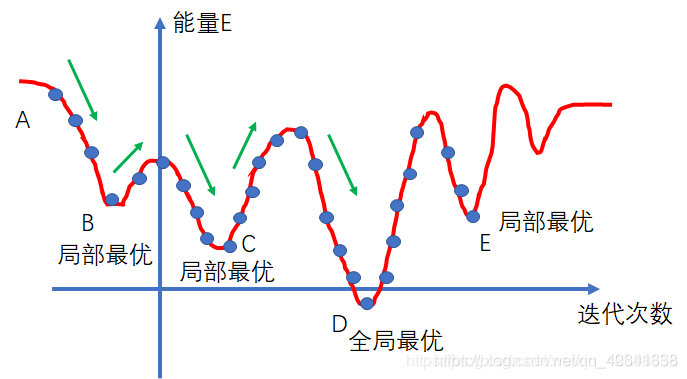
\includegraphics[scale=0.382]{pix/Boltzmann/simulated_annealing.png}
\caption{Simulated Annealing}
\label{fig:simulated_annealing}
\end{figure}

如上图\ref{fig:simulated_annealing} 所示,为模拟退火算法的示意图,在梯度下降法中,
算法只有“下坡”的能力,没有“爬坡”的能力。而模拟退火算法不仅具有“下坡”能力,还赋予其爬坡能力。


%+++++++++++++++++++++++++++++++++++++++++++
\subsection{Boltzmann distribution}

在热力学中,对于一个封闭的系统,温度越高,混乱程度就越高,当温度降低时,
系统逐渐趋于热力学平衡状态。对应神经网络的最优解。

将模拟退火算法和玻尔兹曼分布同 Hopfield 神经网络结合起来,
就可以得到一种基于概率的神经网络模型 —— Boltzmann 机,其有以下特点:

\begin{itemize}
%\setlength{\itemsep}{0pt}
%\setlength{\parsep}{0pt}
\setlength{\parskip}{0pt}
\item[-]
初始温度可以设置得较高,使其拥有足够的“爬坡”能力;

\item[-]
在迭代的过程中,温度逐渐降低,知道最终趋于最小温度(即网络达到平衡状态)

\item[-]
在迭代降低温度时,降低的速率应该足够慢,可以采用线性更替:$T(n+1)=\eta T(n)$,$0.8<\eta<0.99$。
\end{itemize}

\begin{figure}[H]
\centering
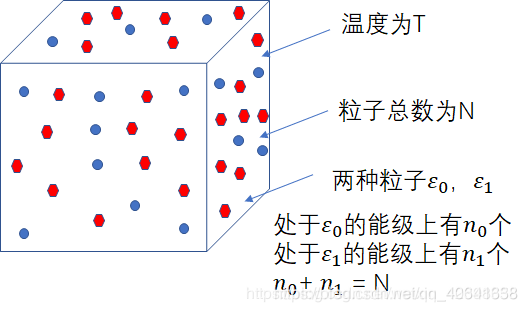
\includegraphics[scale=0.382]{pix/Boltzmann/Boltzmann_distribution.png}
\caption{Boltzmann distribution}
\label{fig:Boltzmann_distribution}
\end{figure}


%+++++++++++++++++++++++++++++++++++++++++++
\section{Boltzmann machine}
%-------------------------------------------

Boltzmann 机是将模拟退火算法和玻尔兹曼分布结合到传统神经网络中构成的一种随机型神经网络模型。
它基本解决了由梯度下降法带来的局部最优问题。但是,它也有很大的缺陷:下面我们由其训练过程可以知道,
Boltzmann 机训练过程时间漫长,所以它在实际中运用的并不多。这促使着大家开始解决由这种 Boltzmann 
机带来的问题,并提出了受限 Bolzmman 机模型。


%+++++++++++++++++++++++++++++++++++++++++++
\subsection{Boltzmann 机的结构}

BM 网络的拓扑结构比较特殊,介于 DHNN 网的全互连结构与 BP 网的层次结构之间。从形式上看,BM 
网络与单层反馈网络 DHNN 网相似,具有对称权值,即,且=0。但从神经元的功能上看,BM 网络与三层 BP 
网相似,具有输人节点、隐节点和输节点称为可见节点,而将隐节点称为不可见节点。
训练时输人输出节点接收训练集样本,而隐节点主要起辅助作用,用来实现输人与输出之间的联系,
使训练集能在可见单元再现。BM网络的三类节点之间没有明显的层次,连接形式可用上图的有向图表示。

\begin{figure}[H]
\centering
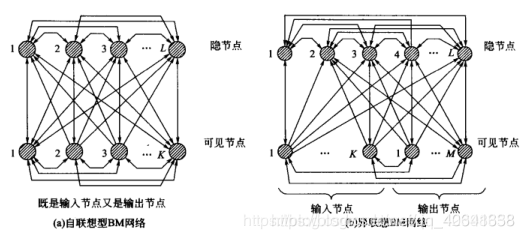
\includegraphics[scale=0.382]{pix/Boltzmann/Boltzmann_machine_architecture.png}
\caption{Architecture of Boltzmann machine}
\label{fig:Boltzmann_machine_architecture}
\end{figure}

同 Hopfield 神经网络有所不同,Boltzmann 机的节点分为可见节点与隐节点,这说明 Boltzmann 
机的结构介于 Hopfield 神经网络和 BP 神经网络之间。它又分为两种类型:

\begin{itemize}
%\setlength{\itemsep}{0pt}
%\setlength{\parsep}{0pt}
\setlength{\parskip}{0pt}
\item[-]
自联想型BM:输入节点与输出节点公用

\item[-]
异联想型BM:可见节点分为输入节点和输出节点
\end{itemize}

无论哪种类型的BM,都有一个共同的特点:所有的节点全连接,整个网络构成一个无向图。


%+++++++++++++++++++++++++++++++++++++++++++
\subsection{Boltzmann机的训练过程}

通过有导师学习,BM网络可以对训练集中各模式的概率分布进行模拟,从而实现联想记忆.
学习的目的是通过调整网络权值使训练集中的模式在网络状态中以相同的概率再现.
学习过程可分为两个阶段;第一阶段称为正向学习阶段或输入期,即向网络输入一对输人输出模式,
将网络输人输出节点的状态“钳制”到期望的状态,而让隐节点自由活动,
以捕捉模式对之间的对应规律;第二阶段称为反向学习阶段或自由运行期,对于异联想学习,
用输人模式“钳住”输人节点而让隐节点和输出节点自由活动,对于自联想学习,
让可见节点和隐节点都自由活动,以体现网络对输人输出对应规律的模拟情况。
输人输出的对应规律表现为网络达到热平衡时,相连节点状态同时为1的平均概率。
期望对应规律与模拟对应规律之间的差别就表现为两个学习阶段所对应的平均概率的差值,
此差值便作为权值调整的依据。设BM网络隐节点数为m,可见节点数为n,
则可见节点可表达的状态X(对于异联想,X中部分分量代表输人模式,另一部分代表输出模式)共有$2^n$ 种。
设训练集提供了 $P$ 对模式,一般有 $P<n$,训练集用一组概率分布表示各模式对出现的概率:

\noindent
{\bf 1. 网络热平衡状态}

为了统计以上的概率,需要反复使BM网络按模拟退火算法运行并达到热平衡状态,具体如下:
\begin{itemize}
%\setlength{\itemsep}{0pt}
%\setlength{\parsep}{0pt}
\setlength{\parskip}{0pt}
\item[1.1]
在正向学习阶段,用一对训练模式钳住网络的可见节点;在反向学习阶段,用训练模式中的输入部分钳住可见节点中的输入节点。  
\item[1.2]
随机选择自由活动节点j,使其更新状态为  
\item[1.3]
计算节点j状态更新而引起的网络能量变化       
\item[1.4]
若则接受状态更新;当时接受新状态,否则维持原状态。是预先设置的数值,在模拟退火过程中,温度T随时间逐渐降低,根据(3)式的讨论情况a看 ,对于常数,为使 ,必须使即在训练中不断减小,因此网络的爬山能力也是减小的。  
\item[1.5]
所有自由节点全部选择一遍  
\item[1.6]
按事先选定的降温方式降温,退火算法的降温规律没有统一的定论,一般要求初始温度足够高,降温速度充分慢,以保证网络收敛到全局最小,我们在模拟退火算法中给出了两个,现在拿出来:  
\item[1.7]
返回步骤②~⑥直到对所有自由节点均有,此时认为网络已经达到热平衡状态,此状态可供学习算法中统计任意两个节点同时为1的概率使用。    
\end{itemize}

\noindent
{\bf 2. 权值调整算法与步骤}

\begin{itemize}
%\setlength{\itemsep}{0pt}
%\setlength{\parsep}{0pt}
\setlength{\parskip}{0pt}
\item[2.1]
随机设定网络的初始权值
\item[2.2]
正向学习阶段按已知概率向网络输入学习模式。在的约束下按上述模拟退火算法运行网络到热平衡状态,统计该状态下网络中任意两个节点i与j同时为1的概率.
\item[2.3]
反向学习阶段在无约束条件下或者在仅输入节点有约束条件下的运行网络到热平衡状态,统计该状态下网络中任意两节点i与j同时为1的概率.
\item[2.4]
权值调整算法为:
\item[2.5]
重复以上的步骤直到与充分接近
\end{itemize}


%+++++++++++++++++++++++++++++++++++++++++++
\section{Types of Boltzmann Machines}
%-------------------------------------------
% https://www.geeksforgeeks.org/types-of-boltzmann-machines/

There are two types of nodes in the Boltzmann Machine — Visible nodes — those nodes 
which we can and do measure, and the Hidden nodes – those nodes which we cannot or 
do not measure. Although the node types are different, the Boltzmann machine 
considers them as the same and everything works as one single system. The training 
data is fed into the Boltzmann Machine and the weights of the system are adjusted 
accordingly. Boltzmann machines help us understand abnormalities by learning about 
the working of the system in normal conditions.

\begin{figure}[H]
\centering
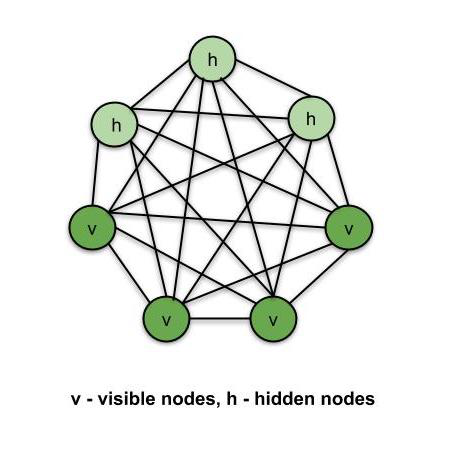
\includegraphics[scale=0.382]{pix/Boltzmann/Boltzmannmachine.jpg}
\caption{Boltzmann Machine}
\label{fig:Boltzmann_Machine}
\end{figure}


%+++++++++++++++++++++++++++++++++++++++++++
\subsection{Energy-Based Models}

{\bf Boltzmann Distribution} is used in the sampling distribution of the Boltzmann 
Machine. The Boltzmann distribution is governed by the equation –
\begin{itemize}
%\setlength{\itemsep}{0pt}
%\setlength{\parsep}{0pt}
\setlength{\parskip}{0pt}
\item[-]
$P_i = e^{(-E_i/kT)} / \sum e^{(-E_j/kT)}$

\item[-]
$P_i$ - probability of system being in state $i$

\item[-]
$E_i$ - Energy of system in state $i$

\item[-]
$T$ - Temperature of the system

\item[-]
$k$ - Boltzmann constant

\item[-]
$\sum e^{(-E_j/kT)}$ - Sum of values for all possible states of the system 
\end{itemize}

Boltzmann Distribution describes different states of the system and thus Boltzmann 
machines create different states of the machine using this distribution. From the 
above equation, as the energy of system increases, the probability for the system 
to be in state ‘$i$’ decreases. Thus, the system is the most stable in its lowest 
energy state (a gas is most stable when it spreads). Here, in Boltzmann machines, 
the energy of the system is defined in terms of the weights of synapses. Once the 
system is trained and the weights are set, the system always tries to find the 
lowest energy state for itself by adjusting the weights.


%+++++++++++++++++++++++++++++++++++++++++++
\subsection{Types of Boltzmann Machines}

\begin{itemize}
%\setlength{\itemsep}{0pt}
%\setlength{\parsep}{0pt}
\setlength{\parskip}{0pt}
\item[-]
Restricted Boltzmann Machines (RBMs)

\item[-]
Deep Belief Networks (DBNs)

\item[-]
Deep Boltzmann Machines (DBMs)
\end{itemize}


%+++++++++++++++++++++++++++++++++++++++++++
\subsection{Restricted Boltzmann Machines (RBMs)}

In a full Boltzmann machine, each node is connected to every other node and hence the 
connections grow exponentially. This is the reason we use RBMs. The restrictions in 
the node connections in RBMs are as follows –
\begin{itemize}
%\setlength{\itemsep}{0pt}
%\setlength{\parsep}{0pt}
\setlength{\parskip}{0pt}
\item[-]
Hidden nodes cannot be connected to one another

\item[-]
Visible nodes connected to one another
\end{itemize}




%+++++++++++++++++++++++++++++++++++++++++++

